%\documentclass[showpacs,superscriptaddress,floatfix,twocolumn,prl]{revtex4}
%\documentclass[11pt,floatfix,notitlepage,amssymb,pra,aps]{revtex4-1}
\documentclass[11pt,floatfix,amssymb,prx,aps,longbibliography,superscriptaddress,nopacs]{revtex4-2}
%\documentclass{amsart}
%\documentclass{report}
%\renewcommand{\familydefault}{cmss}


\usepackage{comment}



%\usepackage[dvipsnames]{xcolor}
\newcommand{\om}{\left( \omega \right)}
\newcommand{\ta}{\tilde{a}\left(\omega\right)}
\newcommand{\tad}{\tilde{a^{\dagger}}\left(\omega\right)}

\newcommand{\tbx}{\tilde{b}_x\left(\omega\right)}
\newcommand{\tbxd}{\tilde{b^{\dagger}}_x\left(\omega\right)}

\newcommand{\tby}{\tilde{b}_y\left(\omega\right)}
\newcommand{\tbyd}{\tilde{b^{\dagger}}_y\left(\omega\right)}


\newcommand{\tZo}{\tilde{Z}\left(\omega\right)}
\newcommand{\tQo}{\tilde{Q}\left(\omega\right)}
\newcommand{\txo}{\tilde{x}\left(\omega\right)}
\newcommand{\tyo}{\tilde{y}\left(\omega\right)}
%\newcommand{\txo}{\tilde{x}_{\scriptscriptstyle{X}}\left(\omega\right)}
%\newcommand{\tyo}{\tilde{x}_{\scriptscriptstyle{Y}}\left(\omega\right)}
\newcommand{\tNx}{\tilde{N}_x\left(\omega\right)}
\newcommand{\tNy}{\tilde{N}_y\left(\omega\right)}
\newcommand{\tNi}{\tilde{N}_i\left(\omega\right)}
\newcommand{\ccm}{\chi_\mathrm{c}^-\left(\omega\right)}
%\newcommand{\cxm}{\chi_x^-\left(\omega\right)}
%\newcommand{\cym}{\chi_y^-\left(\omega\right)}
\newcommand{\cxm}{\chi_x\left(\omega\right)}
\newcommand{\cym}{\chi_y\left(\omega\right)}
\newcommand{\Ix}{\tilde{I}_x\left(\omega\right)}
\newcommand{\Iy}{\tilde{I}_y\left(\omega\right)}

%\newcommand{\Vm}{\boldmath{V}^{\scriptscriptstyle{\mathrm{M}}}}
\newcommand{\Vm}{V^{\scriptscriptstyle{\mathrm{M}}}}
\newcommand{\nm}{\bar{n}}
\newcommand{\nX}{n_{\scriptstyle{x}}}
\newcommand{\nY}{n_{\scriptstyle{y}}}
\newcommand{\OmegaXY}{\Omega_{\scriptstyle{x,y}}}
\newcommand{\OmegaX}{\Omega_{\scriptstyle{x}}}
\newcommand{\OmegaY}{\Omega_{\scriptstyle{y}}}
\newcommand{\OmegaZ}{\Omega_{\scriptstyle{z}}}
\newcommand{\Omegab}{\Omega_{\mathrm{b}}}
\newcommand{\Omegad}{\Omega_{\mathrm{d}}}
\newcommand{\Omegaeff}{\Omega_{\scriptstyle{\mathrm{eff}}}}
\newcommand{\GY}{\Gamma_{\scriptstyle{y}}}
\newcommand{\GX}{\Gamma_{\scriptstyle{x}}}
\newcommand{\GXY}{\Gamma_{\scriptstyle{x,y}}}
\newcommand{\omegaL}{\omega_{\scriptscriptstyle{\mathrm{L}}}}
\newcommand{\gX}{g_{\scriptstyle{x}}}
\newcommand{\gY}{g_{\scriptstyle{y}}}
\newcommand{\gb}{g_{\mathrm{b}}}
\newcommand{\bX}{\hat{b}_{\scriptstyle{x}}}
\newcommand{\bY}{\hat{b}_{\scriptstyle{y}}}
\newcommand{\bdX}{\hat{b}^{\dagger}_{\scriptstyle{x}}}
\newcommand{\bdY}{\hat{b}^{\dagger}_{\scriptstyle{y}}}
\newcommand{\ac}{\hat{a}_{\mathrm{c}}}
\newcommand{\Gm}{\Gamma_{\mathrm{m}}}
\newcommand{\Omegamj}{\Omega_{j}}
\newcommand{\xzpf}{x_{\mathrm{zpf}}}
\newcommand{\pzpf}{p_{\mathrm{zpf}}}
\newcommand{\yzpf}{y_{\mathrm{zpf}}}
\newcommand{\Xc}{\mathrm{X}_{\scriptstyle{\mathrm{c}}}}
\newcommand{\Yc}{\mathrm{Y}_{\scriptstyle{\mathrm{c}}}}
%\newcommand{\xX}{x_{\scriptscriptstyle{X}}}
%\newcommand{\xY}{x_{\scriptscriptstyle{Y}}}
%\newcommand{\pX}{p_{\scriptscriptstyle{X}}}
%\newcommand{\pY}{p_{\scriptscriptstyle{Y}}}
\newcommand{\xX}{x}
\newcommand{\xY}{y}
\newcommand{\pX}{p_{\scriptstyle{x}}}
\newcommand{\pY}{p_{\scriptstyle{y}}}
\newcommand{\ud}{\mathrm{d}}
\newcommand{\blu}[1]{{\color[rgb]{0,0,1}#1}}
\newcommand{\rosso}[1]{{\color[rgb]{1,0,0}#1}}
\newcommand{\verde}[1]{{\color[rgb]{0,1,0}#1}}
\newcommand{\viola}[1]{{\color[rgb]{1,0,1}#1}}

%\newcommand{\xiX}{\xi_{\scriptscriptstyle{X}}}
%\newcommand{\xiY}{\xi_{\scriptscriptstyle{Y}}}
\newcommand{\xiX}{\xi_{\scriptstyle{x}}}
\newcommand{\xiY}{\xi_{\scriptstyle{y}}}

\newcommand{\supp}{s}
\newcommand{\splitt}{\delta}
\newcommand{\cor}{c}

\usepackage{amsmath}
\usepackage[dvips]{graphicx}
\usepackage{epsfig}
\usepackage{tabularx}
\pagestyle{plain}
\usepackage{lineno}
\usepackage{ulem}
\usepackage{xcolor}
\usepackage{soul}
%\linespread{1.6}


\begin{document}



\title[]{Supplementary Material for: High purity two-dimensional levitated mechanical oscillator}



\author{Q. Deplano}
\affiliation{Dipartimento di Fisica e Astronomia, Universit\`a di Firenze, via Sansone 1, I-50019 Sesto Fiorentino (FI), Italy}
\affiliation{INFN, Sezione di Firenze, via Sansone 1, I-50019 Sesto Fiorentino (FI), Italy}

\author{A. Pontin}
\affiliation{CNR-INO, largo Enrico Fermi 6, I-50125 Firenze, Italy}

\author{A. Ranfagni}
\affiliation{Dipartimento di Fisica e Astronomia, Universit\`a di Firenze, via Sansone 1, I-50019 Sesto Fiorentino (FI), Italy}

\author{F. Marino}
\affiliation{CNR-INO, largo Enrico Fermi 6, I-50125 Firenze, Italy}
\affiliation{INFN, Sezione di Firenze, via Sansone 1, I-50019 Sesto Fiorentino (FI), Italy}

\author{F. Marin}
\email[Electronic mail: ]{francesco.marin@unifi.it}
\affiliation{Dipartimento di Fisica e Astronomia, Universit\`a di Firenze, via Sansone 1, I-50019 Sesto Fiorentino (FI), Italy}
\affiliation{European Laboratory for Non-Linear Spectroscopy (LENS), via Carrara 1, I-50019 Sesto Fiorentino (FI), Italy}
\affiliation{INFN, Sezione di Firenze, via Sansone 1, I-50019 Sesto Fiorentino (FI), Italy}
\affiliation{CNR-INO, largo Enrico Fermi 6, I-50125 Firenze, Italy}

%\date{\today}



\maketitle


\tableofcontents
%\doublespacing  




\section*{Model}

The motion in the transverse tweezer plane is described in terms of dimensionless position and momentum operators $\xX, \pX, \xY, \pY$ obtained by normalizing the corresponding physical variables to their respective zero-point fluctuations $\xzpf = \sqrt{\hbar/2 m \OmegaXY}$ and $\pzpf = \sqrt{\hbar m \OmegaXY/2 }$ ($m$ is the mass of the nanosphere, $\OmegaXY$ the oscillation frequencies of the $X$ and $Y$ modes in the absence of optomechanical interaction). The Langevin equations of motion are:
\begin{eqnarray}
\dot{x} & = & \OmegaX \,\pX 
\label{eq_dxdt}\\
\dot{p}_{\scriptstyle{x}} &=& -\OmegaX \,\xX -\gamma_x \,\pX + 2 \gX\, Q + 2 \sqrt{\GX} \,\xiX \\
\dot{y} & = & \OmegaY \,\pY \\
\dot{p}_{\scriptstyle{y}} &=& -\OmegaY \,\xY -\gamma_y \,\pY + 2 \gY \,Q + 2 \sqrt{\GY} \,\xiY \\
\dot{Q} &=& -\Delta P -\frac{\kappa}{2} \,Q + \sqrt{\kappa}\, Q_{\mathrm{in}}  \\
\dot{P} &=& \Delta Q -\frac{\kappa}{2}\, P + 2 \gX \,\xX + 2 \gY\, \xY + \sqrt{\kappa}\, P_{\mathrm{in}}
\label{eq_dPdt}
\end{eqnarray}
where $\,Q\,=\,(a\,+\,a^{\dag})\,$ and  $\,P\,=\,i(a^{\dag}\,-\,a)\,$ are the quadratures of the intracavity field $a$, and $\,Q_{\mathrm{in}}\,=\,(a_{\mathrm{in}}\,+\,a_{\mathrm{in}}^{\dag})\,$,  $\,P_{\mathrm{in}}\,=\,i(a_{\mathrm{in}}^{\dag}\,-\,a_{\mathrm{in}})\,$ are the quadratures of the input vacuum noise. The noise sources have non-null correlation functions $\langle \xiX(t) \, \xiX(t')\rangle = \langle \xiY(t) \, \xiY(t')\rangle = \langle a_{\mathrm{in}}(t) \, a^{\dag}_{\mathrm{in}}(t')\rangle= \delta(t-t')$ (due to the high background temperature, we can classically model the mechanical noise). 

The gas damping rates $\gamma_j$ play a negligible role at low pressure, where optomechanical damping largely dominates, and we fix them at the nominal value of $10^{-4} \,\mathrm{s}^{-1}$. The decoherence of the motion is mainly due to collisions with the background gas, and to quantum noise in the dipole scattered light. The corresponding rates $\GXY$ are left as free parameters in the analysis of the experimental data, and the inferred values well agree, within their uncertainties, with their theoretical estimates \cite{Ranfagni2022}. In particular, for this experiment such agreement is obtained by assuming a background pressure in the range $(2 \div 3) \times 10^{-8}\,$mbar, which is indeed the indication given by two pressure gauges in different positions of the vacuum chamber.  
The optomechanical coupling rates $\gX$ and $\gY$ are proportional to $\sin^2 \theta$ and $\sin \theta \cos \theta$ respectively. Also in this case, we consider them as free parameters in the data analysis, the agreement with the expected values is good \cite{Ranfagni2022}, and from their ratio we deduce the actual angle of the polarization axis. 

From the Langevin equations (\ref{eq_dxdt} - \ref{eq_dPdt}) we derive the drift and diffusion matrices used in the main text for the Lyapunov equation.

The Langevin equations can be written in the Fourier space as
\begin{eqnarray}
\tQo &=& i \ccm \left[g_x \txo+g_y \tyo  \right]+\tilde{Q}_\mathrm{in} \left(\omega\right)
\label{eq_Lang1} \\
\txo &=&  2  \gX \cxm \tQo + \tNx 
\label{eq_Lang2} \\
\tyo &=& 2  \gY \cym \tQo + \tNy 
\label{eq_Lang3}
\end{eqnarray}
where the tilde denotes Fourier transformed (FT) operators $\tilde{O}\left(\omega\right)=\mathrm{FT}\left[\hat{O}\left(t\right)\right]$, and
$\tilde{O}^{\dagger}\left(\omega\right)=\mathrm{FT}\left[\hat{O}^{\dagger}\left(t\right)\right]$.
We have defined the susceptibilities
\begin{eqnarray}
%\chi_x\left(\omega\right)=\frac{\OmegaX}{\OmegaX^2-\omega^2-i\omega\gamma_x}\\
%\chi_y\left(\omega\right)=\frac{\OmegaY}{\OmegaY^2-\omega^2-i\omega\gamma_y}\\
\chi_j\left(\omega\right) &=& \frac{\Omega_j}{\Omega_j^2-\omega^2-i\omega\gamma_j}\\
\chi_\mathrm{c}\left(\omega\right) &=& \frac{1}{-i
\left(\Delta+\omega\right)+\kappa/2}
\end{eqnarray}
with $j= (x, y)$, and the compact form
$\,\ccm=\chi_\mathrm{c}\left(\omega\right) \,-\,
\chi_\mathrm{c}^{*}\left(-\omega\right)$.
The noise input terms can be written as
\begin{gather}
\tilde{Q}_\mathrm{in} \left(\omega\right) = \sqrt{\kappa}\left[\chi_\mathrm{c} \om \tilde{a}_{\mathrm{in}}\om +
\chi_\mathrm{c}^{*} \left(- \omega\right) \tilde{a}^{\dagger}_{\mathrm{in}}\left(  \omega \right)  \right]\\
%\tNx = \sqrt{\GX}\left[\chi_x \om \tilde{b}_{\mathrm{in},x}\om +
%\chi_x^{*} \left(- \omega\right) \tilde{b}^{\dagger}_{\mathrm{in},x}\left(  \omega \right)  \right] \\
%\tNy = \sqrt{\GY}\left[\chi_y \om \tilde{b}_{\mathrm{in},y}\om +
%\chi_y^{*} \left(- \omega\right) \tilde{b}^{\dagger}_{\mathrm{in},y}\left(  \omega \right)  \right]  \, .
\tNi=2 \sqrt{\Gamma_i} \chi_i\om \tilde{\xi}_i   \, .
\end{gather}

We define the bright mode as  $x_\mathrm{b} = \frac{1}{g_\mathrm{b}}\left(\gX x+ \gY y\right)$. Using it in Eq. (\ref{eq_Lang1}) and combining Eqs. (\ref{eq_Lang2}-\ref{eq_Lang3}) we obtain two equations respectively for $\tilde{Q}$ and $\tilde{x}_{\mathrm{b}}$. Inserting the first into the second we derive 
%\begin{equation}
%   \tilde{x}_\mathrm{b} \left( \omega \right)=\frac{1}{g_\mathrm{b}\left[1-2 i \ccm \left( \gX^2 %\chi_x + \gY^2 \chi_y \right) \right]}\Bigl\{2\left(\gX^2\chi_x +\gY^2 \chi_y \right) %\tilde{Q}_\mathrm{in}  \left(\omega\right) +\gX \tNx + \gY \tNy \Bigr\}
%\end{equation}
\begin{equation}
   \tilde{x}_\mathrm{b} \left( \omega \right)=\frac{2\left(\gX^2\chi_x +\gY^2 \chi_y \right) \tilde{Q}_\mathrm{in}  \left(\omega\right) +\gX \tNx + \gY \tNy}{g_\mathrm{b}\left[1-2 i \ccm \left( \gX^2 \chi_x + \gY^2 \chi_y \right) \right]}
\end{equation}
from which we calculate the displacement noise spectrum
\begin{equation}
S_{x_\mathrm{b} x_\mathrm{b}}\om=\frac{4}{\gb^2}\,
\frac{\gX^2 \,\GX \left|\chi_x\right|^2
+\gY^2 \,\GY\left|\chi_y\right|^2+\left|\gX^2 \chi_x+\gY^2 \chi_y\right|^2
\kappa \left|\chi_\mathrm{c}\left(-\omega\right)\right|^2}
{\left|1-2 i \chi_\mathrm{c}^{-}\left(\gX^2 \chi_x+\gY^2 \chi_y\right)\right|^2}
\end{equation}
used in the main text.

The cavity output field is given by the input-output relation 
%$\hat{a} = \sqrt{\kappa} \hat{a}_{\mathrm{c}}-\hat{a}_{\mathrm{in}}$. 
$a_{\mathrm{out}} = \sqrt{\kappa} a-a_{\mathrm{in}}$, and
the heterodyne spectrum normalized to shot noise can be written as
\begin{equation}
S_{\mathrm{out}}(\Omega_{\mathrm{LO}}+\omega) 
= 1 + \eta  \,\kappa \,\left|\chi_\mathrm{c}\left(\omega\right)\right|^2 \,\gb^2 \, S_{x_\mathrm{b} x_\mathrm{b}}\om  \, .
\end{equation}

The parameter $g_{\mathrm{b}}$ plays no meaningful role in the model, and indeed it cancels out in the expression of the heterodyne spectrum. We note however that, by defining it as 
\begin{gather}
g_\mathrm{b}=\sqrt{\frac{\gX^2\Omega_x+\gY ^2 \Omega_y}{\Omega_{\mathrm{b}}}}
\end{gather}
where
\begin{gather}
\Omega_{\mathrm{b}}=\sqrt{\frac{\gX^2 \Omega_{x}^3+\gY^2 \Omega_{y}^3}{\gX^2\Omega_{x}+\gY^2 \Omega_{y}}} 
\label{eq_Omegab}
\end{gather}
and assuming that $\gX \propto \sin^2 \theta$ and $\gY \propto \sin \theta \cos \theta$, $x_{\mathrm{b}}$ can be identified as the motion along the cavity axis, normalized to the zero-point fluctuations $\sqrt{\hbar/2 m \Omega_{\mathrm{b}}}$.

\subsection*{Ground state probability}

If the correlations between the two mechanical modes are negligible, the probability of the two-dimensional ground state is simply given by $1/(\nX+1)(\nY+1)$, and it is larger than 0.25 whenever both thermal occupancies are below unity. In the general case this expression is not valid, but the ground state probability can be calculated from the covariance matrix, with an integration on the phase-space. Defining the vector of phase-space variables $R=(x,\, p_x,\, y,\, p_y)$, the Wigner function of the two-dimensional Gaussian state is \cite{Paris2003}
\begin{equation}
    W(R) = \frac{1}{(2\pi)^2\,\sqrt{\mathrm{Det}[\Vm]}}\,\exp\left(-\frac{1}{2} R (\Vm)^{-1} R^{\mathrm{T}}\right)
\end{equation}
and the projector on the two-dimensional ground state, expressed in the phase-space, is 
\begin{equation}
g(R) = 4 \exp \left(-\frac{1}{2} R\,R^{\mathrm{T}}\right)  \, .
\end{equation}
Finally, the probability that the two-dimensional oscillator is in its ground state is given by
\begin{equation}
    \mathrm{P}(0,0) = \int W(R)\,g(R)\, \mathrm{d}^4R  \,.
\end{equation}
The calculated ground state probability for our system is reported in Table \ref{Tab_Suppl_2}.

\subsection*{Quantum discord of a bipartite Gaussian state}

The quantum discord is calculated for a two-mode squeezed thermal state in Ref.
 \cite{Giorda2010}, 
and for a general bipartite Gaussian state in Ref.
\cite{Adesso2010}. 
A simplified expression is given in Ref. 
\cite{Olivares2012}. 
For the sake of completeness, we report below its full evaluation starting from our definition of phase-space operators.

The covariance matrix $\Vm$ can be written using 2x2 blocks {\boldmath $\alpha$}, {\boldmath $\beta$} and {\boldmath $\gamma$} in the form
\begin{displaymath}
    \Vm_{\scriptstyle{\phi}} = 
    \left( \begin{array}{cc}
    \mbox{\boldmath $\alpha$} & \mbox{\boldmath $\gamma$} \\
    \mbox{\boldmath $\gamma$}^{\scriptstyle{T}}  &  \mbox{\boldmath $\beta$}
    \end{array}  \right)
\end{displaymath}
The correlations between the orthogonal modes are contained in the off-diagonal  block {\boldmath $\gamma$}.

Four symplectic invariants are defined as $I_1=\mathrm{Det}[\mbox{\boldmath $\alpha$}]$, $I_2=\mathrm{Det}[\mbox{\boldmath $\beta$}]$, $I_3=\mathrm{Det}[\mbox{\boldmath $\gamma$}]$, and $I_4=\mathrm{Det}[\Vm]$. With our definitions, describing a physical system requires $\,I_1, I_2 \ge 1\,$ and $\,d_{\pm} \ge 1$, where the symplectic eigenvalues are defined by 
% $\,d_{\pm} = \sqrt{\frac{D \pm \sqrt{D^2-4 I_4}}{2}}\,$
$\,d_{\pm} = \sqrt{(D \pm \sqrt{D^2-4 I_4} ) /2}\,$ 
with $D = I_1+I_2+2 I_3$. 

If $\,(I_4- I_1 I_2)^2\le (1+I_2) I_3^2 (I_1+I_4)\,$ (a condition which is verified in our case), the quantum discord can be calculated as
\begin{equation}
    \mathcal{D}_{X \leftarrow Y}\,=\,f\left(\sqrt{I_2}\right)-f\left(d_{+}\right)-f\left(d_{-}\right)+f\left(E\right)
\end{equation}
where 
\begin{equation}
    f(x) = \frac{x+1}{2} \,\log{\left(\frac{x+1}{2}\right)}-\frac{x-1}{2} \,\log{\left(\frac{x-1}{2}\right)}
\end{equation}
($\log$ is the natural logarithm) and
\begin{equation}
    E\,=\,\frac{|I_3| + \sqrt{I_3^2+\left(I_2-1\right)\left(I_4-I_1\right)}}{I_2-1}   \, .
\end{equation}
The expression of $\mathcal{D}_{Y \leftarrow X}$ is obtained from that of $\mathcal{D}_{X \leftarrow Y}$ by swapping $I_1$ and $I_2$.

\subsection*{Quantum discord in a rotated frame  }

To define the phase-space in a geometrically rotated frame, we must consider that the modal eigenfrequency depends on the direction (see Eq.
\ref{eq_Omegab}) 
and therefore also the zero-point fluctuations used to normalize the position and momentum variables. However, the symplectic invariants of the covariance matrix do not depend on this normalization.
We then removed the normalization to the zero-point fluctuations of the $X$ and $Y$ modes, avoiding to rely on their uncoupled resonance frequencies $\OmegaXY$, and computed the covariance matrix of the mechanical system in an arbitrary reference frame as $\Vm_{\scriptstyle{\phi}} = R(\phi) N \Vm N R^{\scriptstyle{T}}(\phi)$. Here $R(\phi)$ rotates by an angle $\phi$ around the $Z$ axis, and $N=\mathrm{Diag}[1/\sqrt{\Omega_x}, \sqrt{\Omega_x}, 1/\sqrt{\Omega_y}, \sqrt{\Omega_y}]$. The quantum discord $\,\mathcal{D}_{\phi \,\leftarrow (\phi+\pi/2)} $ is calculated from $\Vm_{\scriptstyle{\phi}}$. 

\section*{Additional data set}

Thanks to a pair of ring electrodes positioned on the tweezer optics holder at about $1\,$mm from the nanosphere, we can generate a static electric field along the tweezer axis. Since the nanosphere is generally charged \cite{Deplano2024}, this allows us to displace its equilibrium position. In this way, we slightly tune the oscillation frequencies and, compensating for the tweezer radiation pressure, maximize the frequency splitting between $X$ and $Y$. 

We acquired two additional data sets, at different applied voltages. Unfortunately, in these data sets the signals given by the rotational motion are more evident, and we had to post-select the time series in order to delete the time intervals in which the erratic rotational peaks cross the spectral regions of interest. The overall signal-to-noise ratio is therefore lower than in the spectra described in the main text. 

\begin{figure}[!htb]
    \centering
      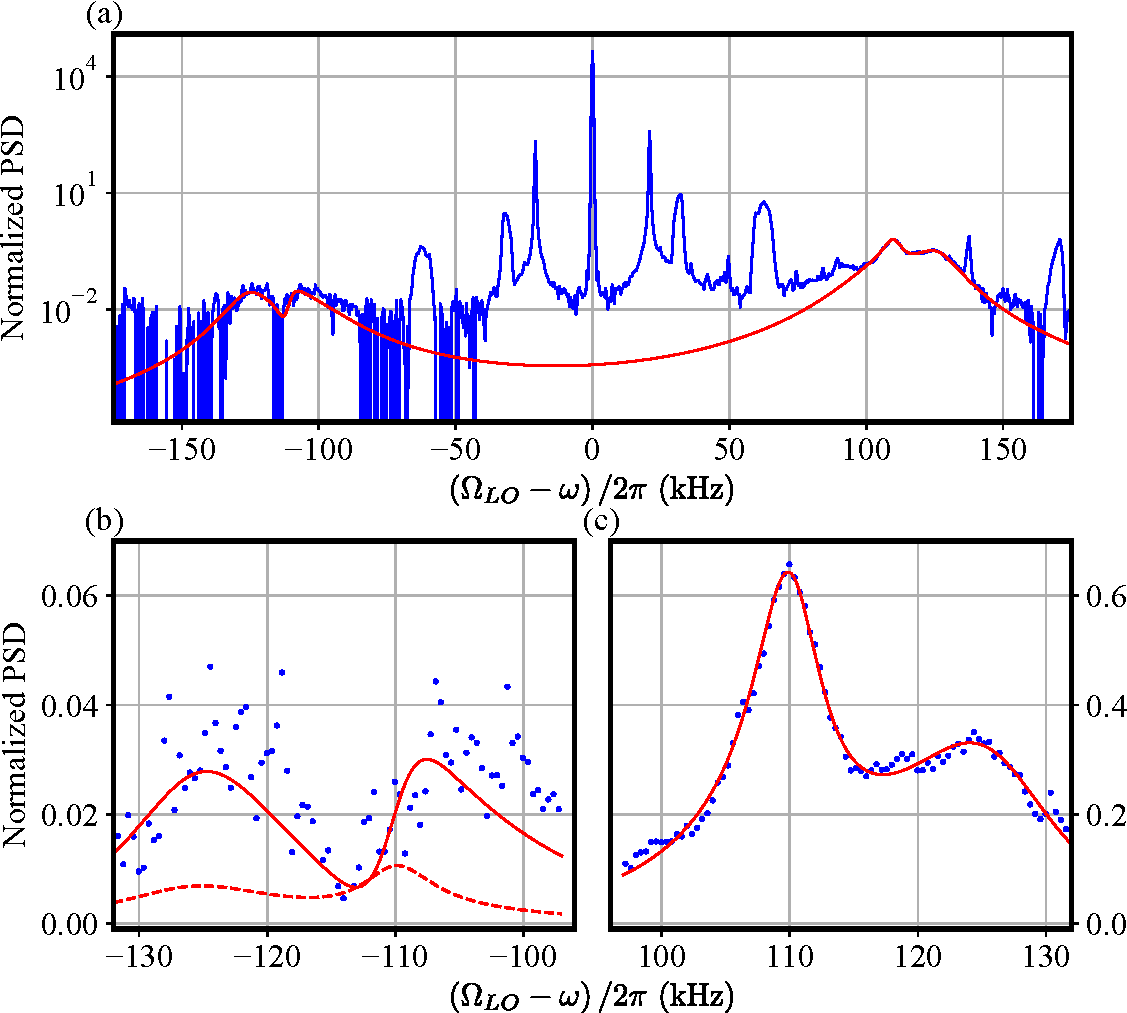
\includegraphics[scale=0.65]{figure_84-188_v3.pdf}
    \caption[Fig2]{\textbf{Power Spectral Density of the heterodyne signal for an additional data set.} The spectrum is normalized to the measured shot noise which is then subtracted (the dark noise is preliminarily subtracted from all spectra). The abscissa is the frequency difference with respect to the local oscillator. The detuning is $\Delta/2\pi = -110\,$kHz, and a voltage of $35\,$V is applied to the electrodes on the tweezer. The red solid line shows the fit of Eqs. (\ref{eq_Sout}-\ref{eq:Sxb}) to the experimental right sideband.  The lower panels display enlarged views of the left (b) and right (c) sidebands. The dashed red line in panel (b) is obtained by replacing $S_{x_\mathrm{b} x_\mathrm{b}}\om\,\to\,S_{x_\mathrm{b} x_\mathrm{b}}\left( -\omega \right)$.}
    \label{Fig_Suppl}
\end{figure}

An example is shown in Fig. \ref{Fig_Suppl}. In panel (b) of the figure, which displays an enlarged view of the left sideband, we also report, together with the theoretical curve fitted to the right sideband, the same theoretical signal with $S_{x_\mathrm{b} x_\mathrm{b}}\om \to S_{x_\mathrm{b} x_\mathrm{b}}\left( -\omega \right)$. It shows how the heterodyne signal would appear in the case of a mechanical system dominated by classical noise, i.e., when the displacement noise spectrum is frequency symmetric and the difference between the two motional sidebands is due exclusively to the cavity filtering. The huge difference, both in amplitude and shape, compared to the actual spectral signal is further evidence of the highly quantum nature of the two-dimensional oscillator.   

In Table \ref{Tab_Suppl_1} we summarize the fitted parameters for all data sets (including the first one, discussed in the main text), and in Table \ref{Tab_Suppl_2} we report the extracted values of several physical quantities characterizing the two-dimensional system.

\begin{table}
\begin{tabular}{c||c|c|c}
Voltage  (V)  &  0 & 22.5 & 35\\
  $\OmegaX/2\pi$ (Hz)  &  $122170\pm120$ & $122290\pm280$ & $121610\pm160$ \\
   $\OmegaY/2\pi$ (Hz)   &  $109370\pm150$ & $108970\pm220$ & $107640\pm150$ \\
 $\gX/2\pi$ (Hz)    & $14130\pm220$ & $14420\pm230$ & $15160\pm310$ \\
   $\gY/2\pi$ (Hz)   &  $10370\pm160$ & $10300\pm190$ & $10060\pm 110$ \\
 $\GX/2\pi$ (Hz)    &  $4030\pm200\pm120$ & $3890\pm220\pm150$ & $3250\pm180\pm100$ \\
  $\GY/2\pi$ (Hz)    & $3050\pm170\pm90$ & $2990\pm160\pm70$ & $2520\pm140\pm70$ \\
\end{tabular}
\caption{Parameters extracted from the fit of three data sets with the model of Eqs. (\ref{eq_Sout}-\ref{eq:Sxb}). The reported uncertainty is the spread (one standard deviation) on five independent acquisitions. For the decoherence rate, the second quoted error derives from a spread of $5\%$ in the detection efficiency, which is a conservative estimate of the uncertainty of an independent measurement yielding $\eta = 0.32$.}
\label{Tab_Suppl_1}
\end{table}

\begin{table}
\begin{tabular}{c||c|c|c}
Voltage  (V)  &  0 & 22.5 & 35\\
  $\nX$  &  $0.551\pm0.003\pm0.027$ & $0.514\pm0.001\pm0.026$ & $0.407\pm0.002\pm0.020$ \\
   $\nY$    &  $0.740\pm0.013\pm0.036$ & $0.716\pm0.007\pm0.036$& $0.626\pm0.007\pm0.031$  \\
 purity   & $0.209\pm0.002\pm0.011$ & $0.219\pm0.002\pm0.011$ & $0.260\pm0.002\pm0.012$ \\
 $\mathcal{D}_{X \leftarrow Y}$ & $0.0423\pm0.0003\pm0.0004$ & $0.0361\pm0.0010\pm0.0006$ & $0.0415\pm0.0011\pm0.0008$ \\
 $\mathcal{D}_{Y \leftarrow X}$ & $0.0471\pm0.0006\pm0.0006$ & $0.0399\pm0.0018\pm0.0004$  & $0.0449\pm0.0016\pm0.0007$  \\
 P(0,0) & $0.386\pm0.003\pm0.014$ & $0.449\pm0.002\pm0.014$ & $0.399\pm0.003\pm0.014$
\end{tabular}
\caption{Thermal occupancies of the $X$ and $Y$ modes considered as one-dimensional oscillators, two-dimensional state purity, quantum discord, and probability of the two-dimensional ground state P(0,0), deduced for three different data sets. The first reported uncertainty is the statistical spread over five independent acquisitions (one standard deviation), the second quoted error derives from an uncertainty of $5\%$ in the detection efficiency.}
\label{Tab_Suppl_2}
\end{table}


%\bibliographystyle{apsrev4-2} 
\bibliography{database}



\end{document}